\documentclass[CMPE]{KGCOEReport}
\usepackage{float}
\usepackage{adjustbox}
\graphicspath{ {./images/} }

\newcommand{\name}{Mohammed Fareed \\ Trent Wesley}
\newcommand{\exerciseNumber}{3}
\newcommand{\exerciseDescription}{Characterization of OPB745}
\newcommand{\dateDone}{September 13, 2023}
\newcommand{\dateSubmitted}{September 20, 2023}

\newcommand{\classCode}{CMPE 460}
\newcommand{\LabSectionNum}{1}
\newcommand{\LabInstructor}{Prof.\ Hussin Ketout}
\newcommand{\TAs}{Andrew Tevebaugh \\ Ben Hyman \\ Colin Vo \\ Marshal Tiechman}
\newcommand{\LectureSectionNum}{1}
\newcommand{\LectureInstructor}{Prof.\ Hussin Ketout}


\begin{document}
\maketitle

\section*{Abstract}

In this laboratory exercise, the OPB745 photo-transducer was characterized by its ability to accurately measure the distance between it and a reflective surface. A test environment made of PVC pipes was made to isolate the sensor from outside light and adjust the distance between the OPB745 photo-transducer and aluminum foil used as a reflective surface. The distance of the reflective surface was varied from 0cm to 50cm. It was found that the voltage drop started high (around 5V) at 0mm indicating that no light was detected. The voltage drop reached a minimum at 5mm indicating that the light intensity detected was strongest at this distance. The voltage drop increased as the distance increased until about 45mm. A function generator was attached to the input of the 7406 inverter and frequency was increased from 100Hz until the output no longer resembled a square wave. It was found that the output waveform stopped resembling a square wave at around 1.2kHz with the 10k$\Omega$ load resistor and around 850Hz with the 20k$\Omega$ resistor.

\section*{Design Methodology}

To set up this exercise, a test environment was built to isolate the OPB745 sensor from outside light. This environment also provided the ability to change the distance between the OPB745 sensor and a reflective surface of aluminum foil inside, with measurement of the distance between them. A diagram of the test environment from the CMPE-460 manual is shown in Figure \ref{fig:env}.

\begin{figure}[H]
    \centering
    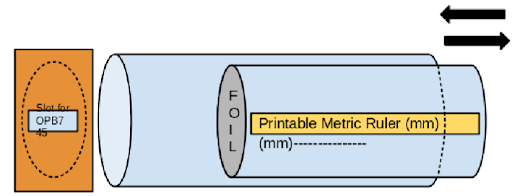
\includegraphics[width=0.75\textwidth]{test_env.png}
    \caption{Test Environment Diagram}
    \label{fig:env}
\end{figure}

The test environment was built out of two PVC pipes. One pipe had a reflective aluminum surface on one end and could be slid into the other pipe with a larger diameter. A metric ruler was added to the inside of the inner pipe for measurement. A slot made of cardboard and tape was added to the end of the larger pipe through which the OPB745 sensor was placed.\\

The first part of this exercise tested the ability of the OPB745 to accurately measure the distance between it and a reflective surface with a 10k$\Omega$ and a 20k$\Omega$ load resistor. The circuit for this part is shown in Figure \ref{fig:circuit1}. This circuit contains an OPB745 which emits and measures light. The value of R$_\text{f}$ was calculated to ensure that the diode receives a proper current. The value of R$_\text{f}$ was calculated using the forward voltage and the continuous forward current of the diode in the OPB745, which were retrieved from the data sheet of the sensor. The following is the calculation of the resistance of R$_\text{f}$:

\[ \frac{5\text{V} - \text{V}_\text{F}}{\text{I}_\text{F}} = \frac{5\text{V} - 1.70\text{V}}{40 \text{mA}} = 82.5 \Omega \]

This circuit was tested with the load resistor equal to 10k$\Omega$ and 20k$\Omega$. The voltage at the V$_{\text{out}}$ node was measured for select distances from 0mm to 50mm and the current across the load resistor was calculated.

\begin{figure}[H]
    \centering
    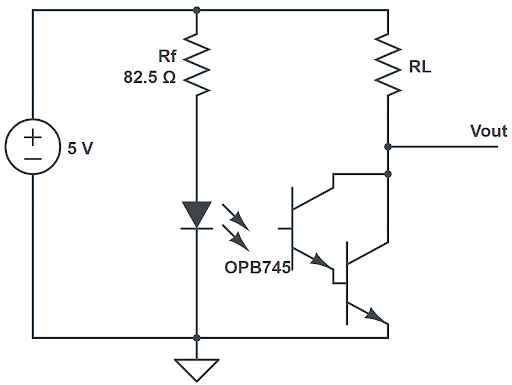
\includegraphics[width=0.5\textwidth]{circuit_1.png}
    \caption{Part 1 Circuit}
    \label{fig:circuit1}
\end{figure}

The second part of this exercise tested how well the output would retain its square wave characteristics as the frequency of a waveform generator was increased. The circuit for this part is shown in figure \ref{fig:circuit2}.

\begin{figure}[H]
    \centering
    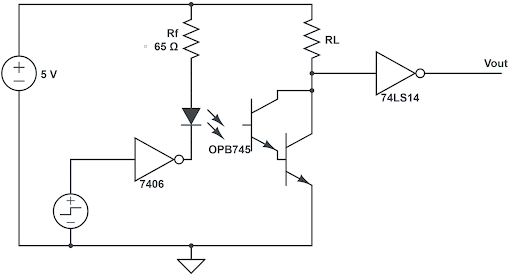
\includegraphics[width=0.75\textwidth]{circuit_2.png}
    \caption{Part 2 Circuit}
    \label{fig:circuit2}
\end{figure}

As shown in Figure \ref{fig:circuit2}, a waveform generator is attached to the input of an inverter. This inverter controls the current that will flow through the LED. Light from the LED hits the phototransistor and causes current to flow through the phototransistor. If enough current flows through the phototransistor, voltage at the input of the Schmitt trigger (74LS14) will be low causing V$_{\text{out}}$ to be high. If not much light hits the phototransistor, minimal current will pass through it. This means that the voltage at the input of the Schmitt trigger will be high and V$_{\text{out}}$ will be low. The resistance of R$_\text{f}$ was calculated using the same method as in part 1, taking into account the voltage drop across the inverting buffer (7406). The value of the voltage drop of the inverting buffer used is its low-output voltage retrieved from the data sheet. The following is the calculation of the resistance of R$_\text{f}$:

\[ \frac{5\text{V} - \text{V}_\text{F} - \text{V}_\text{OL}}{\text{I}_\text{F}} = \frac{5\text{V} - 1.70\text{V} - 0.70\text{V}}{40 \text{mA}} = 65 \Omega \]

The waveform generator was initially set to 100Hz with a duty cycle of 50\%. The frequency was increased by increments of 100Hz until the output no longer retained its square wave characteristics. The frequency at which the output no longer resembled a square wave was recorded. This was repeated with the load resistor equal to 10k$\Omega$ and 20k$\Omega$.

\section*{Results and Analysis}

Part 1 of this exercise consisted of increasing the distance between the OPB745 and the reflective surface. 10k$\Omega$ and 20k$\Omega$ load resistors were tested and the voltage at V$_{\text{out}}$ was measured. Table \ref{table:data} shows the distances tested and the output voltage, for each load resistance. The current across the load resistor was calculated using Ohm's law as follows:

\[ I_{RL} = \frac{5\text{V} - V_{\text{out}}}{R_L} \]

The table shows that $V_{\text{out}}$ starts at 5V and then decreases sharply to a minimum as the sensor is no longer in contact with the reflective surface. The voltage then increases gradually as the distance increases and less light is reflected back to the sensor. The calculated current across the load resistor shows the inverse relationship between the voltage and current. The current starts at around 0A, sharply increases to a maximum, and then decreases gradually as the distance increases. At 45mm, the voltage starts to decrease again (and the current increases) likely due to the test environment not being completely isolated towards the end of the pipe.

\begin{table}[H]
    \centering
    \caption{Results of Part 1}
    \begin{tabular}{|c|c|c|c|c|}
        \hline
        & \multicolumn{2}{|c|}{$R_{L1} = 10k\Omega$} & \multicolumn{2}{|c|}{$R_{L1} = 20k\Omega$} \\
        \hline
        Distance (mm) & $V_{\text{out}}$ (V) & $I_{RL}$ (mA) & $V_{\text{out}}$ (V) & $I_{RL}$ (mA) \\
        \hline
        0 & 4.98 & 0.002 & 4.96 & 0.002 \\
        \hline
        1 & 1.65 & 0.335 & 2.61 & 0.1195 \\
        \hline
        2 & 0.73 & 0.427 & 0.68 & 0.216 \\
        \hline
        3 & 0.67 & 0.433 & 0.53 & 0.2235 \\
        \hline
        4 & 0.63 & 0.437 & 0.17 & 0.2415 \\
        \hline
        5 & 0.62 & 0.438 & 0.17 & 0.2415 \\
        \hline
        6 & 0.64 & 0.436 & 0.19 & 0.2405 \\
        \hline
        7 & 0.67 & 0.433 & 0.55 & 0.2225 \\
        \hline
        8 & 0.69 & 0.431 & 0.64 & 0.218 \\
        \hline
        9 & 0.71 & 0.429 & 0.67 & 0.2165 \\
        \hline
        10 & 0.72 & 0.428 & 0.69 & 0.2155 \\
        \hline
        11 & 0.74 & 0.426 & 0.70 & 0.22 \\
        \hline
        12 & 0.75 & 0.425 & 0.72 & 0.214 \\
        \hline
        13 & 0.76 & 0.424 & 0.73 & 0.2135 \\
        \hline
        14 & 0.77 & 0.423 & 0.74 & 0.213 \\
        \hline
        15 & 0.79 & 0.421 & 0.75 & 0.2125 \\
        \hline
        20 & 0.87 & 0.413 & 0.80 & 0.21 \\
        \hline
        25 & 2.45 & 0.255 & 0.86 & 0.207 \\
        \hline
        30 & 3.28 & 0.172 & 1.98 & 0.151 \\
        \hline
        35 & 3.77 & 0.123 & 2.80 & 0.11 \\
        \hline
        40 & 3.96 & 0.104 & 2.90 & 0.11 \\
        \hline
        45 & 3.96 & 0.104 & 2.96 & 0.102 \\
        \hline
        50 & 3.65 & 0.135 & 2.60 & 0.12 \\
        \hline
    \end{tabular}
    \label{table:data}
\end{table}

The voltage and current were plotted for both load resistors, as shown in Figure \ref{fig:plots}.

\begin{figure}[H]
    \centering
    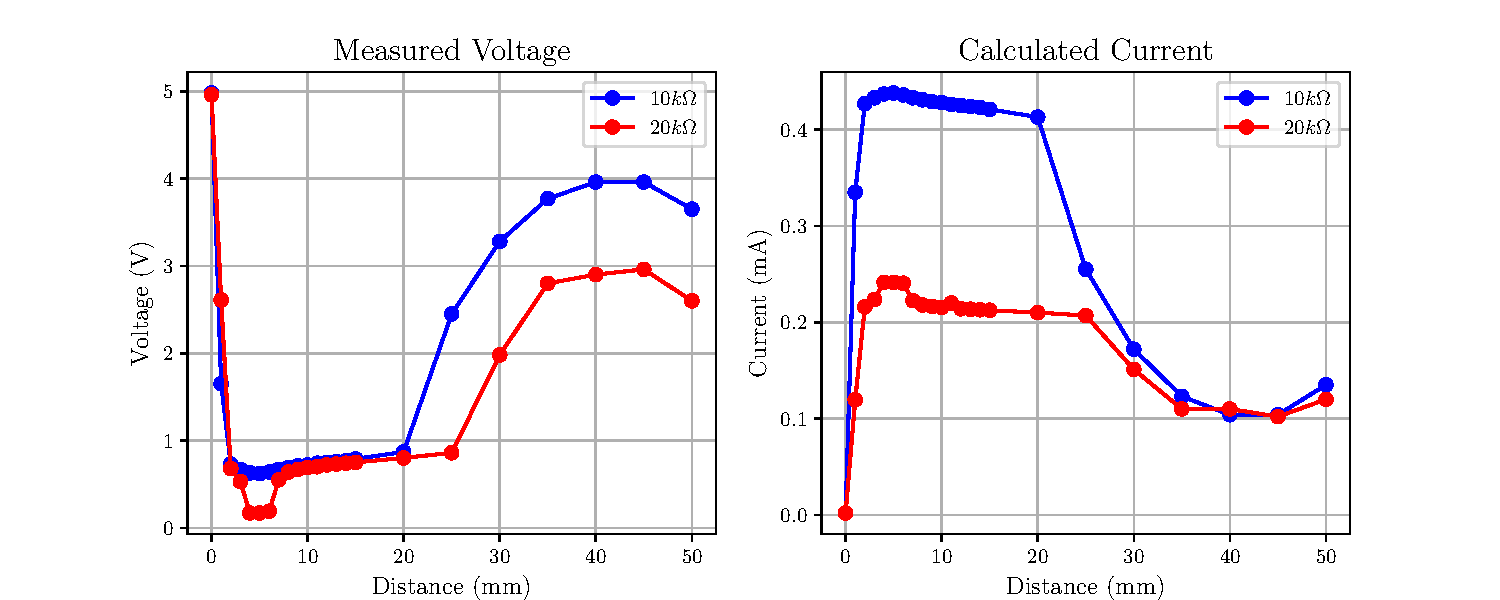
\includegraphics[width=1\textwidth]{results_plot.pdf}
    \caption{Plotted Part 1 Results}
    \label{fig:plots}
\end{figure}

The plots show that the change in the load resistance affects both the voltage and current characteristics of the circuit. The increase in the load resistance decreases both the maximum voltage across the phototransistor and the current passing through the load. \\

Part 2 consisted of increasing the frequency of the waveform generator until the output no longer resembled a square wave. Figure \ref{fig:osc_10_min} shows the input (green) of the waveform generator and the output V$_\text{out}$ (yellow). Figure \ref{fig:osc_10_max} shows the results at 1.2kHz.

\begin{figure}[H]
    \centering
    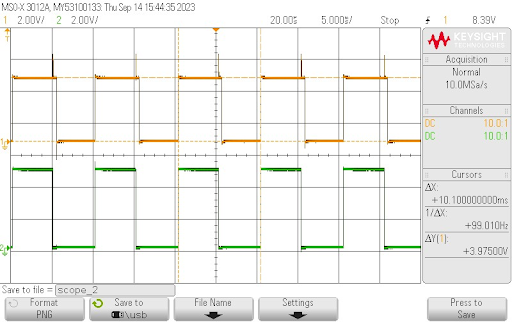
\includegraphics[width=0.75\textwidth]{output_min_10.png}
    \caption{Oscilloscope Capture with 10k$\Omega$ Load Resistor at 100Hz.}
    \label{fig:osc_10_min}
\end{figure}

\begin{figure}[H]
    \centering
    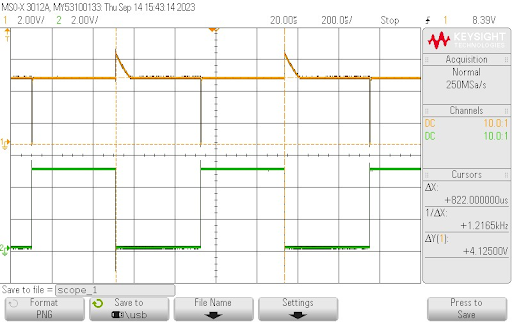
\includegraphics[width=0.75\textwidth]{output_max_10.png}
    \caption{Oscilloscope Capture with 10k$\Omega$ Load Resistor at 1.2kHz.}
    \label{fig:osc_10_max}
\end{figure}

Around 1.2kHz, the output no longer resembled a square wave as the duty cycle was almost 100\%, resembling a DC signal. The output in both Figure \ref{fig:osc_10_min} and Figure \ref{fig:osc_10_max} shows a spike in the output, which was attributed to noise. \\

Figures \ref{fig:osc_20_min} and \ref{fig:osc_20_max} show the results of the same test with a 20k$\Omega$ load resistor. The output no longer resembled a square wave at around 850Hz and the spike in the output was still present.

\begin{figure}[H]
    \centering
    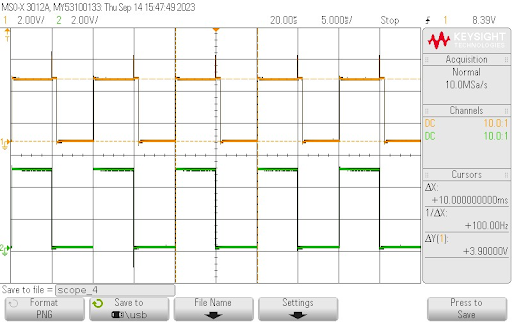
\includegraphics[width=0.75\textwidth]{output_min_20.png}
    \caption{Oscilloscope Capture with 20k$\Omega$ Load Resistor at 100Hz.}
    \label{fig:osc_20_min}
\end{figure}

\begin{figure}[H]
    \centering
    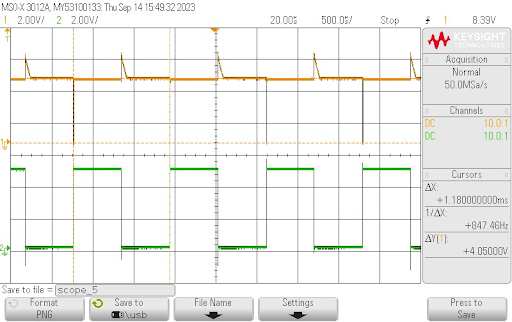
\includegraphics[width=0.75\textwidth]{output_max_20.png}
    \caption{Oscilloscope Capture with 20k$\Omega$ Load Resistor at 850Hz.}
    \label{fig:osc_20_max}
\end{figure}

\section*{Questions}

1. \emph{In the lab we do not use a 7406 inverter on the output; instead we use the 74LS14 with Schmitt trigger. Why do we need to do this, and what is the difference between the two?}

The 74LS14 is used to convert the output of the OPB745 to a conditioned square wave. The difference between the two is that the 74LS14 Schmitt trigger will introduce hysteresis in the process of converting the signal to a square wave, while the 7406 inverter will not. The hysteresis reduces the noise in the output signal and makes the output more stable. It is introduced by having two different threshold voltage levels for logic high and logic low voltages of the input signal.
\bigskip

2. \emph{Why does the voltage start at 5V at 0mm and then drop quickly? Why does it eventually go back to 5V?}

At 0mm, the sensor is in contact with the reflective surface, and thus senses no light. At the point it is no longer in contact with the reflective surface, it gets the maximum amount of light, resulting in the drop of voltage. As the sensor is moved away from the reflective surface, the amount of light absorbed by the sensor starts decreasing, increasing the voltage gradually.
\bigskip

3. \emph{Why does the frequency change when going from a 10K load resistor to a 20K load resistor? Did you anticipate it increasing or decreasing and why?}

When the resistance is increased, the time constant $\tau=RC$ increases, causing a greater delay in the charging and discharging of the capacitor forming between the resistor and phototransistor. This causes the input frequency required to cause the output to approach 100\% duty cycle to decrease. We anticipated the frequency to decrease because as the resistance increases and the time constant increases, it requires less frequency to cause the phototransistor to not have enough time to shut off before the next cycle begins, thus staying in the HIGH state (100\% duty cycle).

\section*{Conclusion}

In this laboratory exercise, the OPB745 photo-transducer was characterized by its ability to accurately measure the distance between it and a reflective surface. A test environment made of PVC pipes was made to isolate the sensor from outside light and adjust the distance between the OPB745 photo-transducer and aluminum foil used as a reflective surface. The distance of the reflective surface was varied from 0cm to 50cm. It was found that the voltage drop started high (around 5V) at 0mm indicating that no light was detected. The voltage drop reached a minimum at 5mm indicating that the light intensity detected was strongest at this distance. The voltage drop increased as the distance increased until about 45mm. A function generator was attached to the input of the 7406 inverter and frequency was increased from 100Hz until the output no longer resembled a square wave. It was found that the output waveform stopped resembling a square wave at around 1.2kHz with the 10k$\Omega$ load resistor and around 850Hz with the 20k$\Omega$ resistor.

\newpage
\begin{figure}[H]
    \centering
    \begin{adjustbox}{center}
        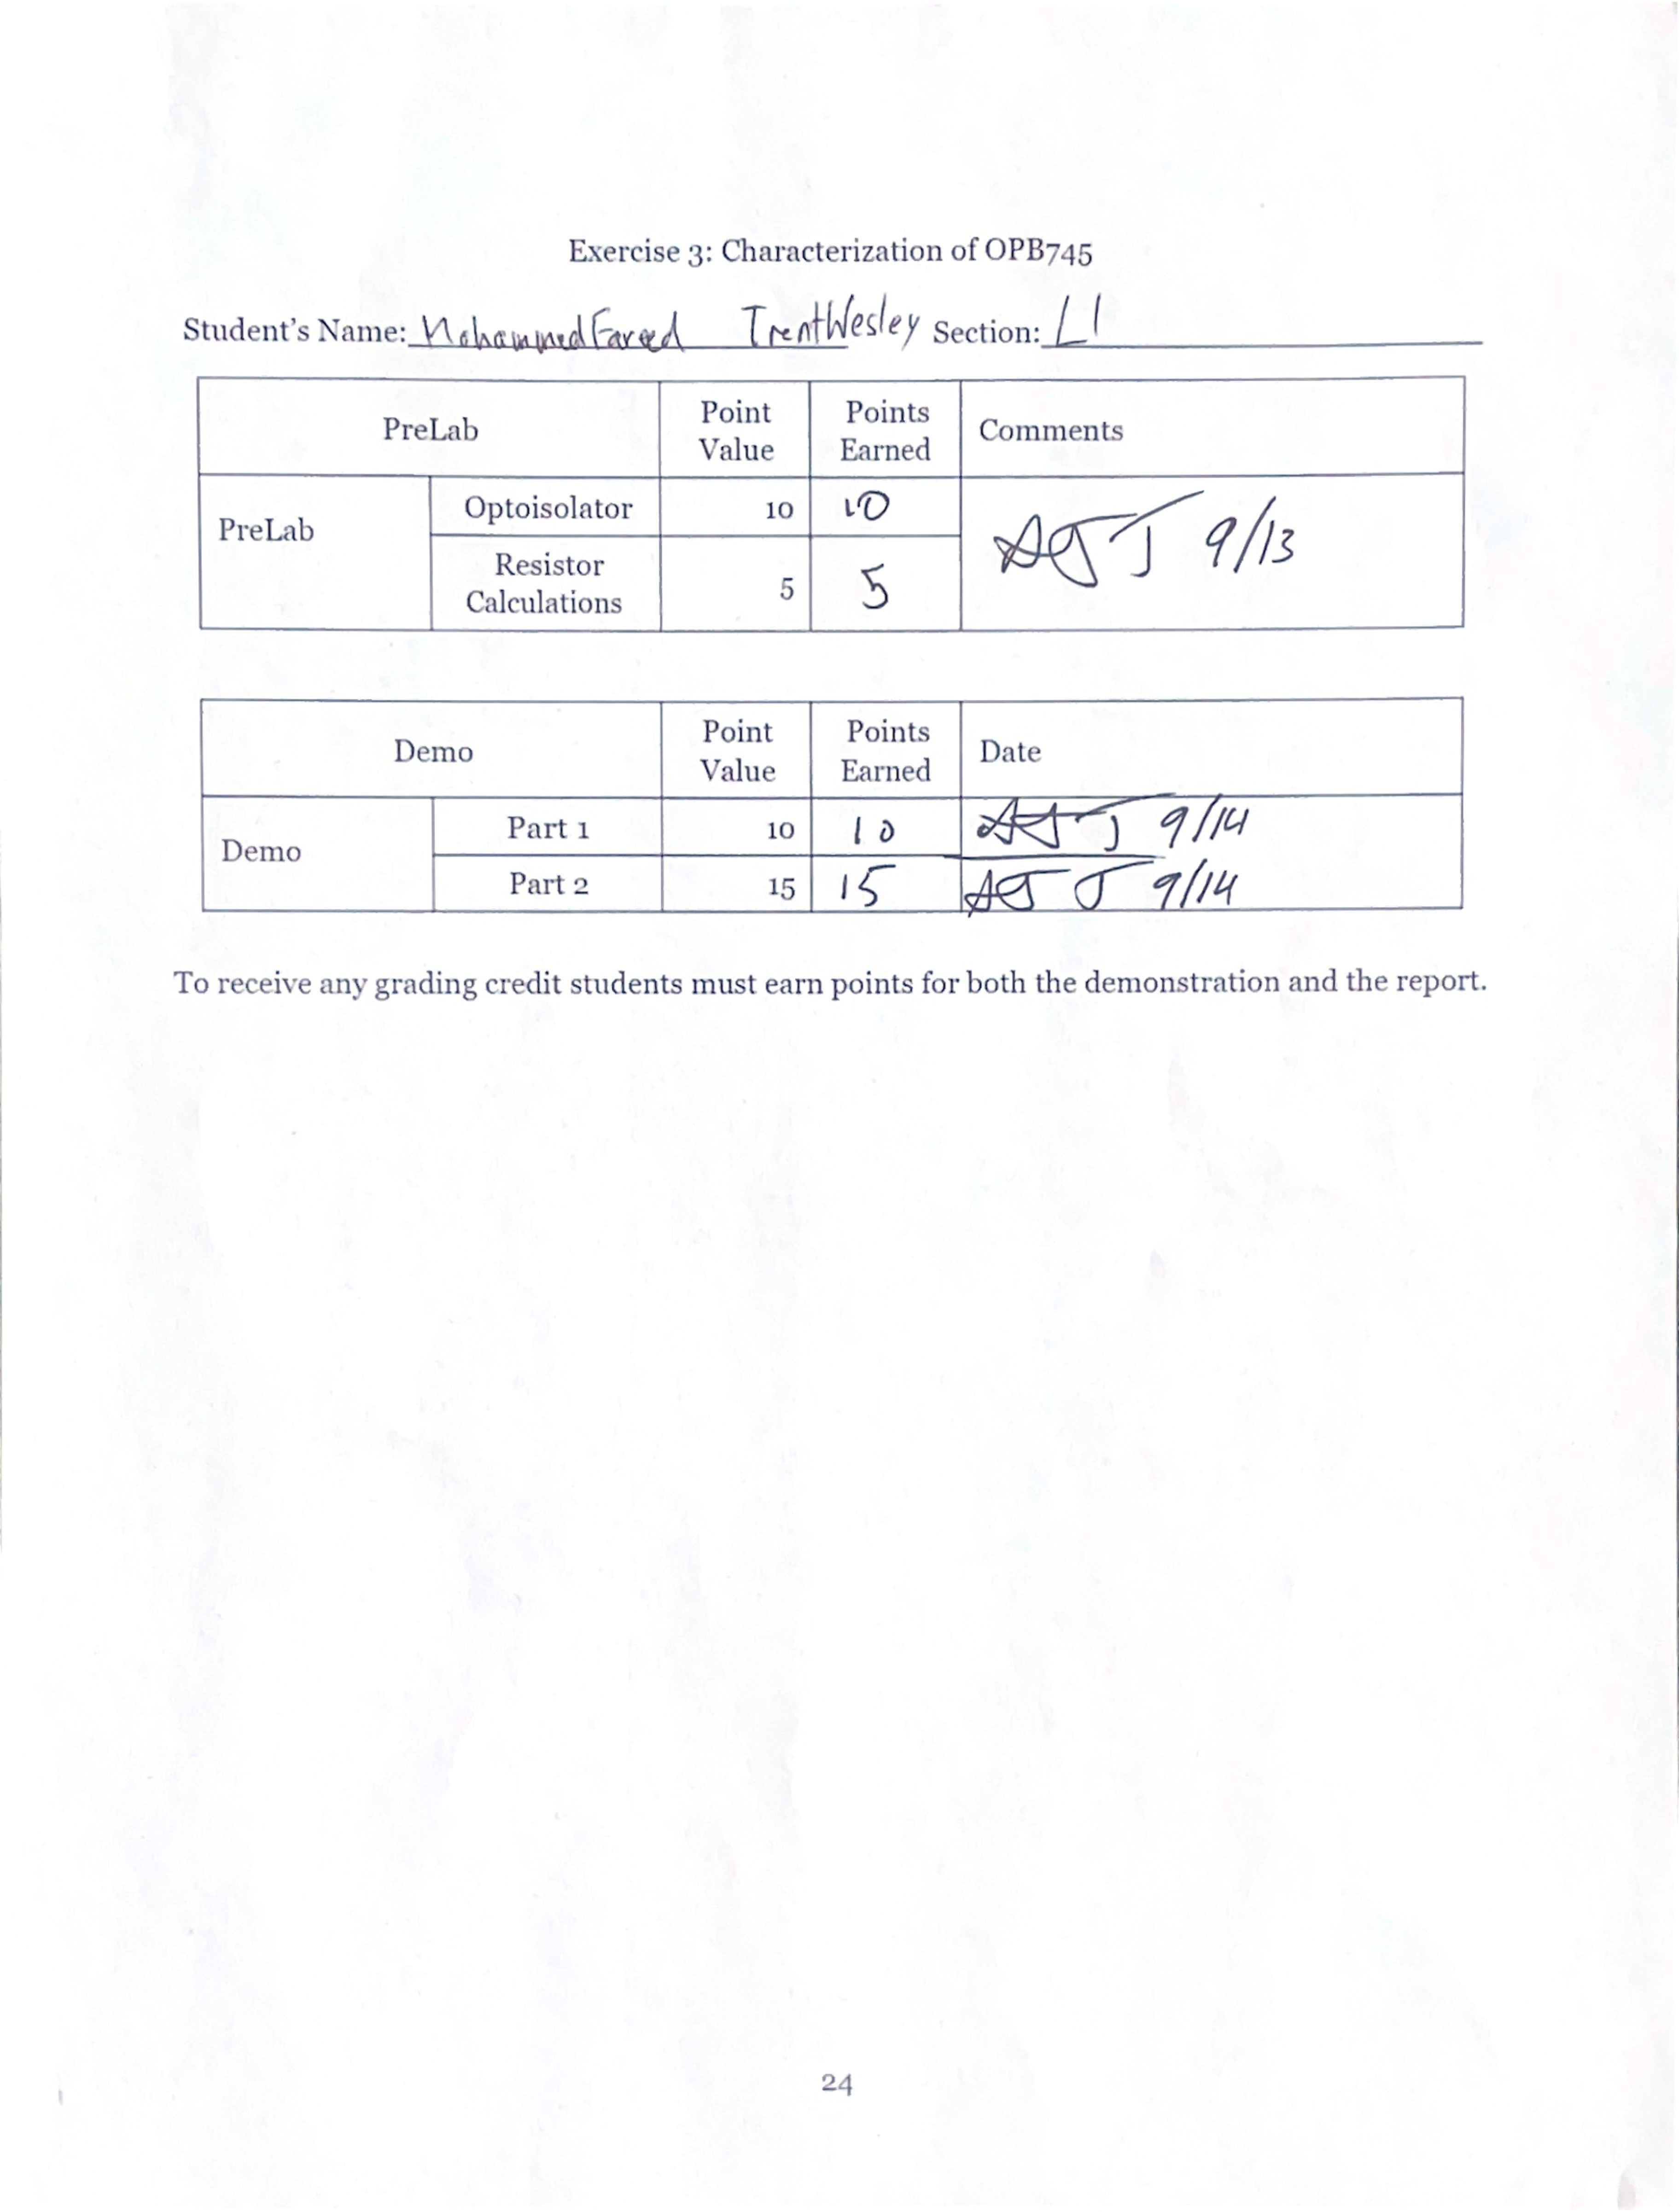
\includegraphics[width=1.35\textwidth]{signoff.pdf}
    \end{adjustbox}
\end{figure}

\end{document}
